\subsection{Naive Cosine Similarity Comparison}

The first approach I tried was to compare the cosine distance between words in the codeword corpus $C_c$ and reference corpus $C_r$. In essence, for each word $w_{i, c}$ in $C_c$, I find $w_{i, r} = w_{i, c}$ in the reference corpus and find $cossim(w_{i, c}, w_{i, r})$ for all words $i$ that are common to both corpora. The idea is that if ``hello'' is not a codeword, then $cossim(w_{hello, c}, w_{hello, r})$ should be similar to the average of all cosine similarities for all words in the corpus (\textbf{I do assume that codewords take up a very minority portion of the codeword entire vocabulary}). However, if ``cheeseburger'' is a codeword, then $cossim(w_{cheeseburger, c}, w_{cheeseburger, r})$ should be far from the mean of the cosine similarity of all words in the corpus. Then, if we plot the $cossim(w_{i, c}, w_{i, r})$ for all words $i$ in the vocabulary that is common to both corpora, then ideally I should observe a mainly normal distribution with codewords falling outside the normal distribution.

\begin{figure}[H]
\centering
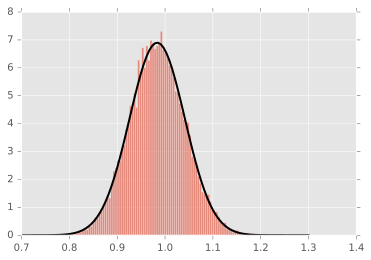
\includegraphics[width=.5\textwidth]{figures/naive-cosine-dist.pdf}
\caption{Distribution of $cossim(w_{i, c}, w_{i, r})$ for all words $i$ in the common vocabulary between $C_c$ and $C_r$ where $C_c$ is the enron corpus and $C_r$ is the 20 news group corpus}
\label{fig-naive-cosine-dist}
\end{figure}

However, this was not observed. Instead, a simple normal distribution was observed as shown in Figure \ref{fig-naive-cosine-dist}. This then required me to have a cutoff Z score for defining codewords. When I took words that are significantly different from the mean with p-value < 0.05, the words found were insignificant and unlikely to be codewords as shown in Figure \ref{fig-naive-cosine-dist-words}.

\begin{figure}[H]
foul, commented, explained, nightline, keeps, yesterday, cummings, mountains, cis, dramatically, ballistic, wishes, spi, encouraged, crash, contention, profound, interview, doubting, rudolf, slider, ray, cracking, chicken, litigation, clogged, brad, unsuccessful, champ, conclusion
\caption{A sample of words that were detected as codewords by using the p-value of 0.05 on the naive cosine distance method}
\label{fig-naive-cosine-dist-words}
\end{figure}

This method clearly did not yield codewords.

\subsection{Word Similarity Comparison}

However, the intuition behind the first method is valuable. After all, the first definition of a codeword is that it is used in a different context as it is usually used. I can approach this problem slightly different -- instead of using the embeddings of the words directly, I can ask for the similar words of a word. For example, for the word ``hello'', the words that are similar to it (i.e. the words that have the highest cosine similarity to the embedding of ``hello'') would be ``hi'', ``bye'' etc. If ``hello'' is not a codeword, we can expect this to be the same in the reference corpus. However, if ``cheeseburger'' was a codeword, the words that are similar to ``cheeseburger'' would be different in both corpus.

Formally, for a given word $w_{i, c}$ in the codeword corpus and $w_{i, r}$ in the reference corpus, we can find the set of words $\mathbf{s_{i, c}}$ that are most similar to $w_{i, c}$ and $\mathbf{s_{i ,r}}$ that are most similar to $w_{i, r}$ in the codeword corpus. I can set $|\mathbf{s_{i, c}}| = |\mathbf{s_{i, r}} = 500$. For example, this would involve me finding the 500 most similar words to ``hello'' in the codeword corpus, then the 500 most similar words to ``hello'' in the reference corpus. Then, I can calculate the intersection of these two sets $\mathbf{s_{i ,c}} \cap \mathbf{s_{i ,r}}$, and count the number of similar words that are shared in both sets (i.e. $|\mathbf{s_{i ,c}} \cap \mathbf{s_{i ,r}}|$). Intuitively, the higher this count is, the more similar the two words are used in both corpuses. Then, a codeword is simply one with a very low similarity count $|\mathbf{s_{i ,c}} \cap \mathbf{s_{i ,r}}|$.

I ran this experiment using the Enron corpus as the codeword corpus, and Wikipedia as the reference corpus. This addresses the issue of words not appearing in the reference corpus encountered earlier. The initial results were promising. For example, I know for sure that ``good'', ``finance'', and ``meeting'' are not codewords in the Enron corpus. These words had similarity counts of 142, 75, and 54 respectively. I also know that ``raptor'' is a codeword in Enron. The similarity count for ``raptor'' is 2.

At this point, before testing the results further, Apoorv and I realized that we needed to find a way to systematically test our results. We needed a synthetic codeword dataset that reflects our definitions of codewords. This can then be used to systematically test our results.